\subsection{Baseline}

\begin{figure}
    
\end{figure}

\subsection{Data augmentation}

\subsection{Threshold}
\begin{figure}
    \centering
    \begin{tabular}{cc}
        \makecell{
            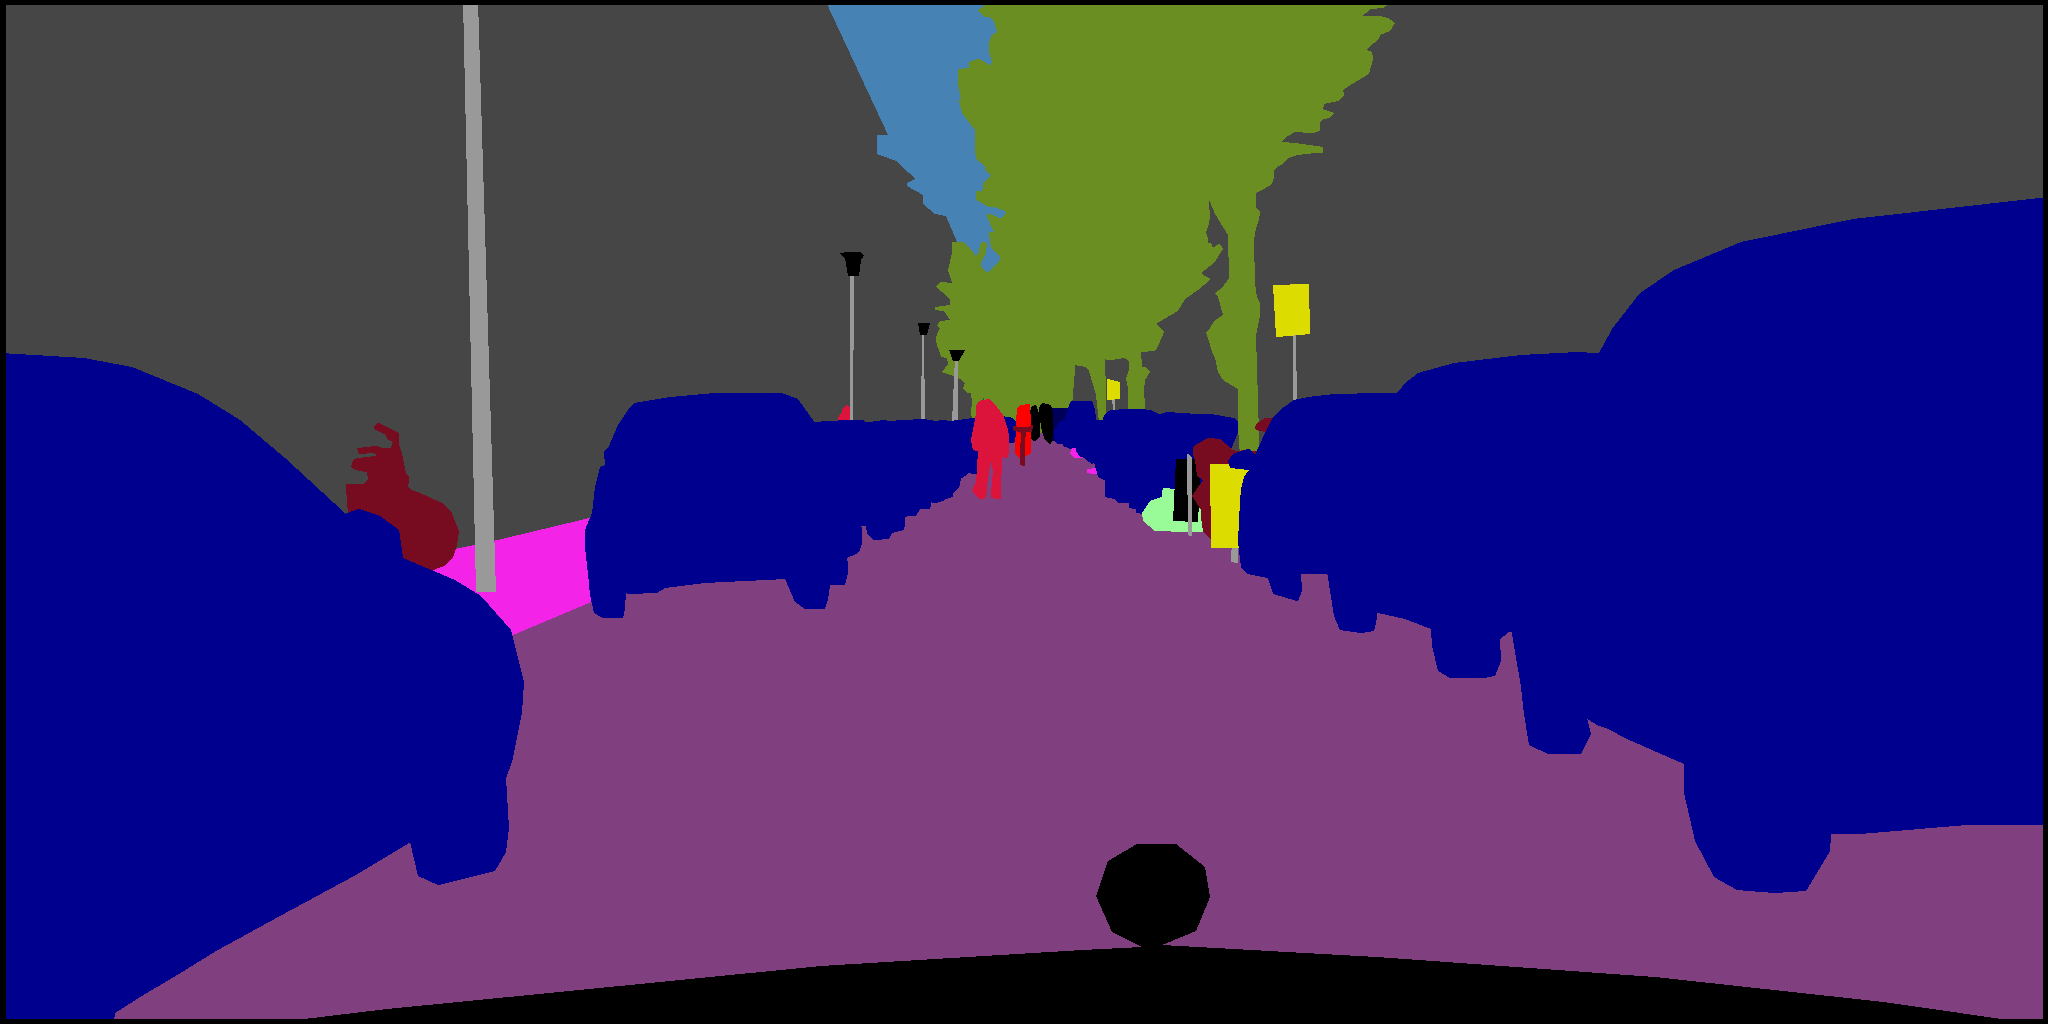
\includegraphics[width=.45\linewidth]{data/threshold/output_truth.png} \\
            Ground Truth 
        } &
        \makecell{
            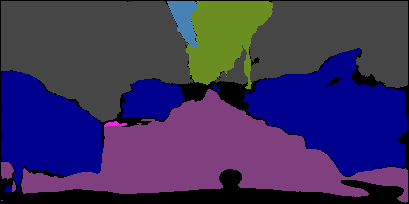
\includegraphics[width=.45\linewidth]{data/threshold/output_1.png} \\
            Epoch 1
        } \\
        \makecell{
            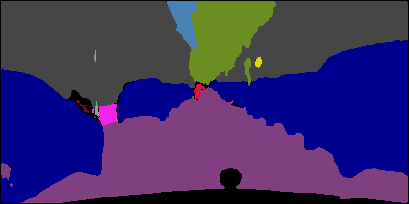
\includegraphics[width=.45\linewidth]{data/threshold/output_5.png} \\
            Epoch 5
        } &
        \makecell {
            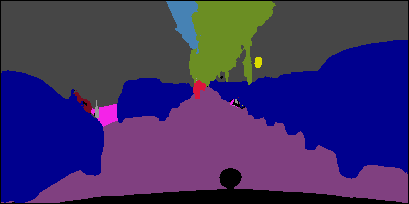
\includegraphics[width=.45\linewidth]{data/threshold/output_10.png} \\
            Epoch 10
        } \\ 
        
    \end{tabular}
    \caption{Ground truth and predicted masks after training for 1, 5 and 10 epochs of the sample \texttt{munster\_000098\_000019\_leftImg8bit.png} using the U-Net model with thresholds and data augmentation}    
\end{figure}

\begin{figure}
    \centering
    \begin{tabular}{cc}
        \makecell{
            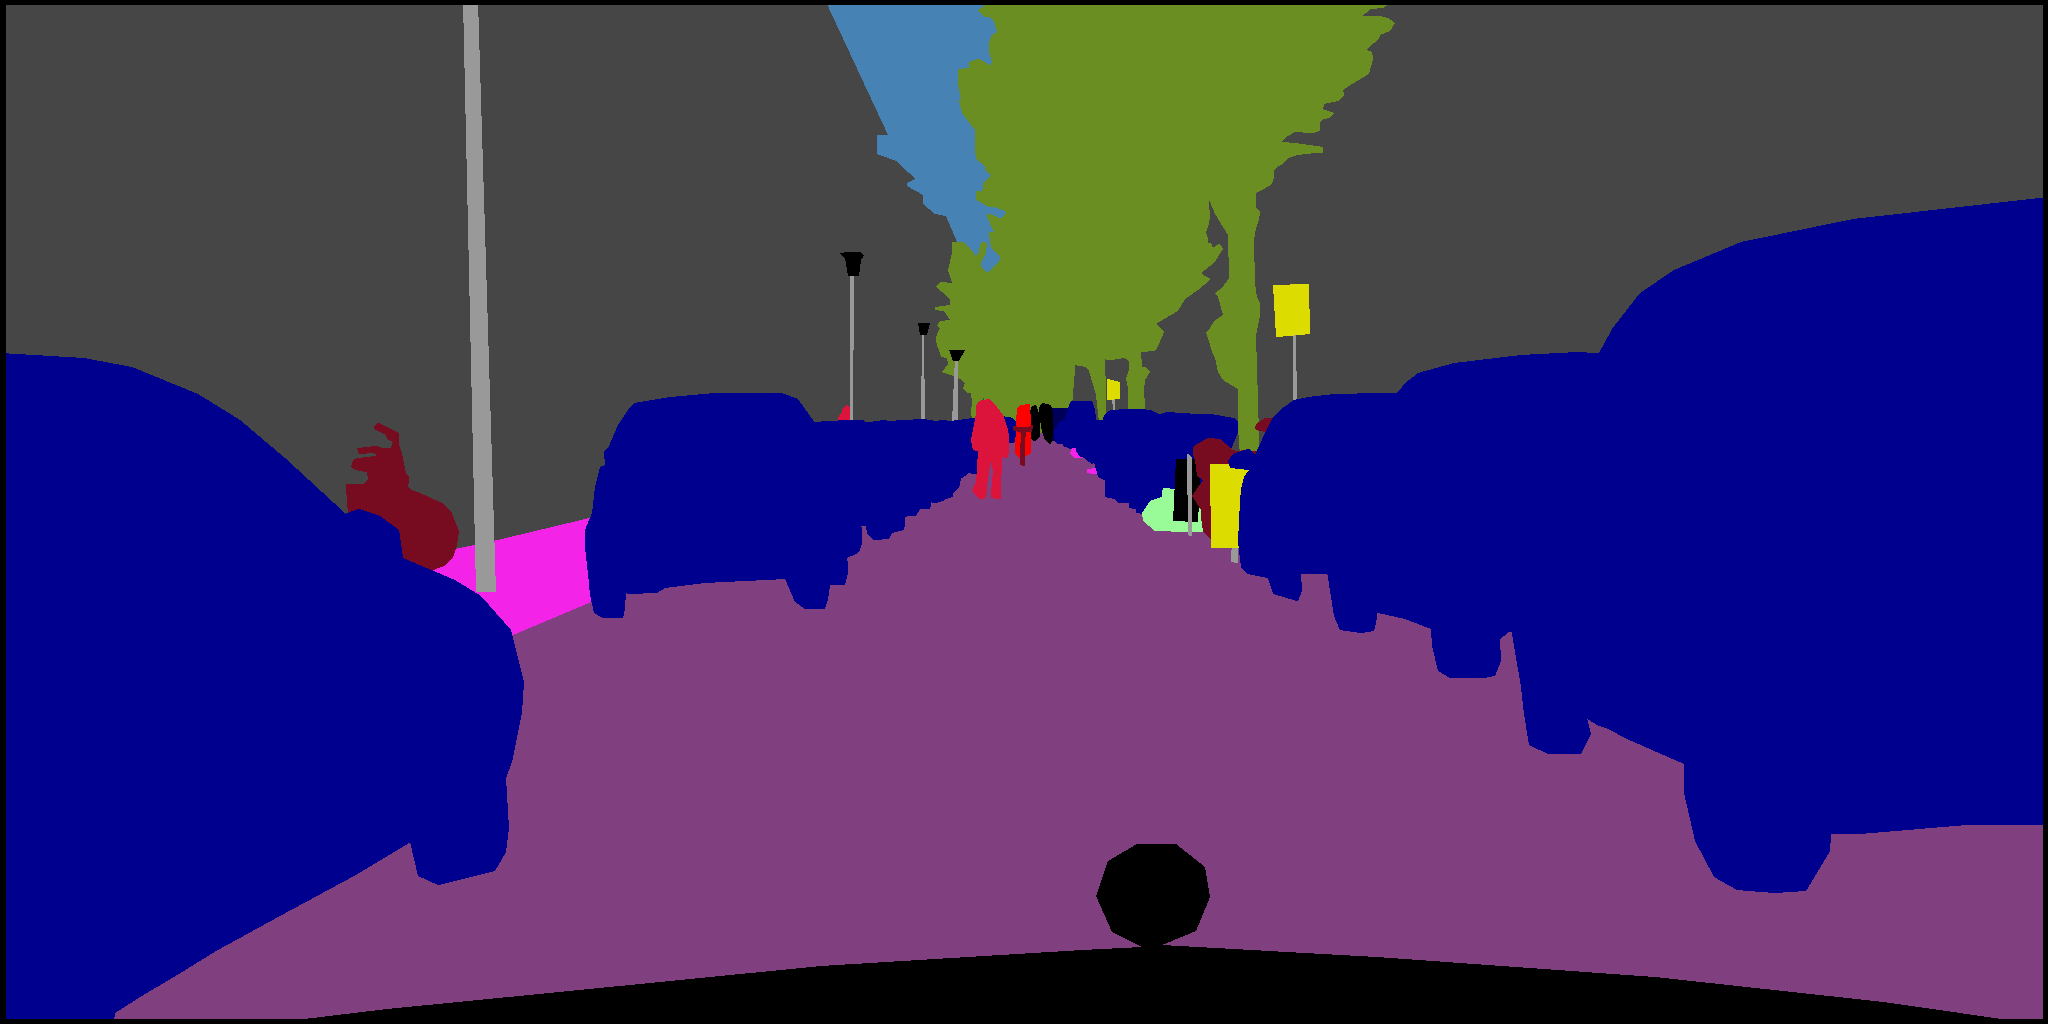
\includegraphics[width=.45\linewidth]{data/threshold/output_truth.png} \\
            Ground Truth 
        } &
        \makecell{
            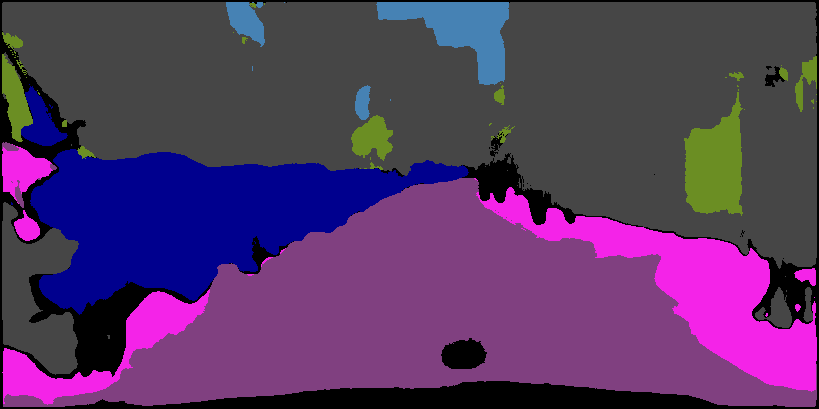
\includegraphics[width=.45\linewidth]{data/reduced-dims/output_1.png} \\
            Epoch 1
        } \\
        \makecell{
            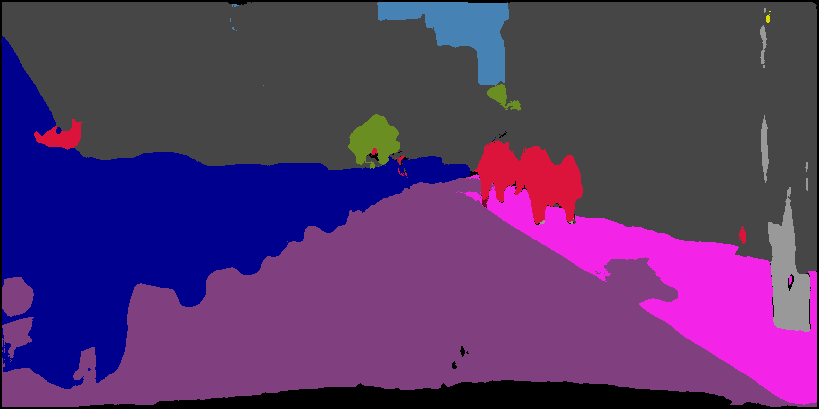
\includegraphics[width=.45\linewidth]{data/reduced-dims/output_5.png} \\
            Epoch 5
        } &
        \makecell {
            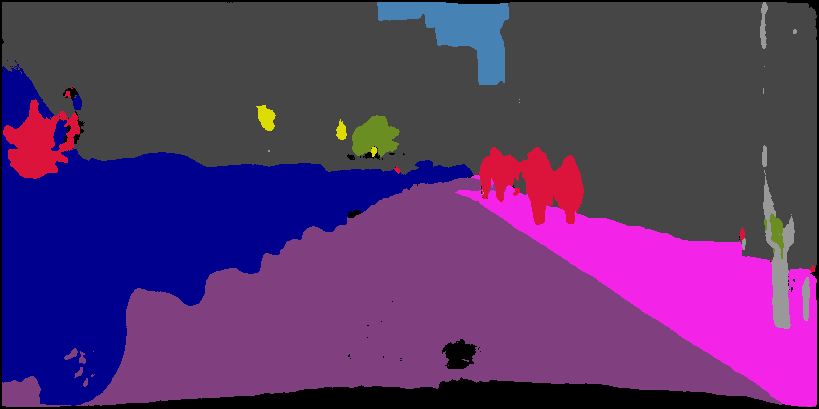
\includegraphics[width=.45\linewidth]{data/reduced-dims/output_10.png} \\
            Epoch 10
        } \\ 
        
    \end{tabular}
    \caption{Ground truth and predicted masks after training for 1, 5 and 10 epochs of the sample \texttt{munster\_000098\_000019\_leftImg8bit.png} using the U-Net model with reduced dimensions}    
\end{figure}